\section{Entwurf}
\subsection{Komponentendiagramm}
Abbildung \ref{fig:Komponentendiagramm} auf Seite \pageref{fig:Komponentendiagramm} zeigt das Komponentendiagramm.

\begin{figure}[htp]
\centering
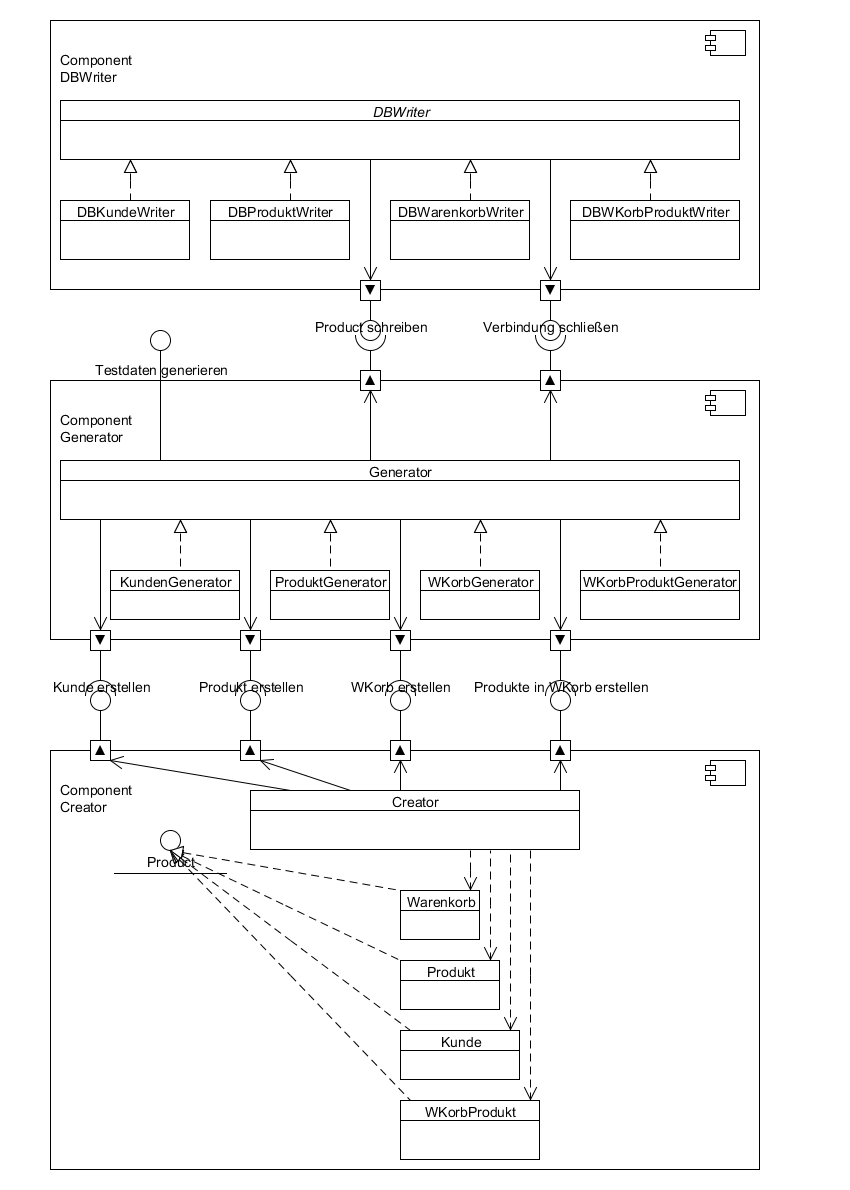
\includegraphics[width=1\textwidth]{Ingo/Bilder/Komponentendiagramm.png}
\caption{Komponentendiagramm}
\label{fig:Komponentendiagramm}
\end{figure}

\subsection{Entwurfsklassendiagramm der Generatorkomponente}
Abbildung \ref{fig:EntwurfGeneratorkomponente} auf Seite \pageref{fig:EntwurfGeneratorkomponente} zeigt das Entwurfsklassendiagramm der Generatorkomponente.

\begin{figure}[htp]
\centering
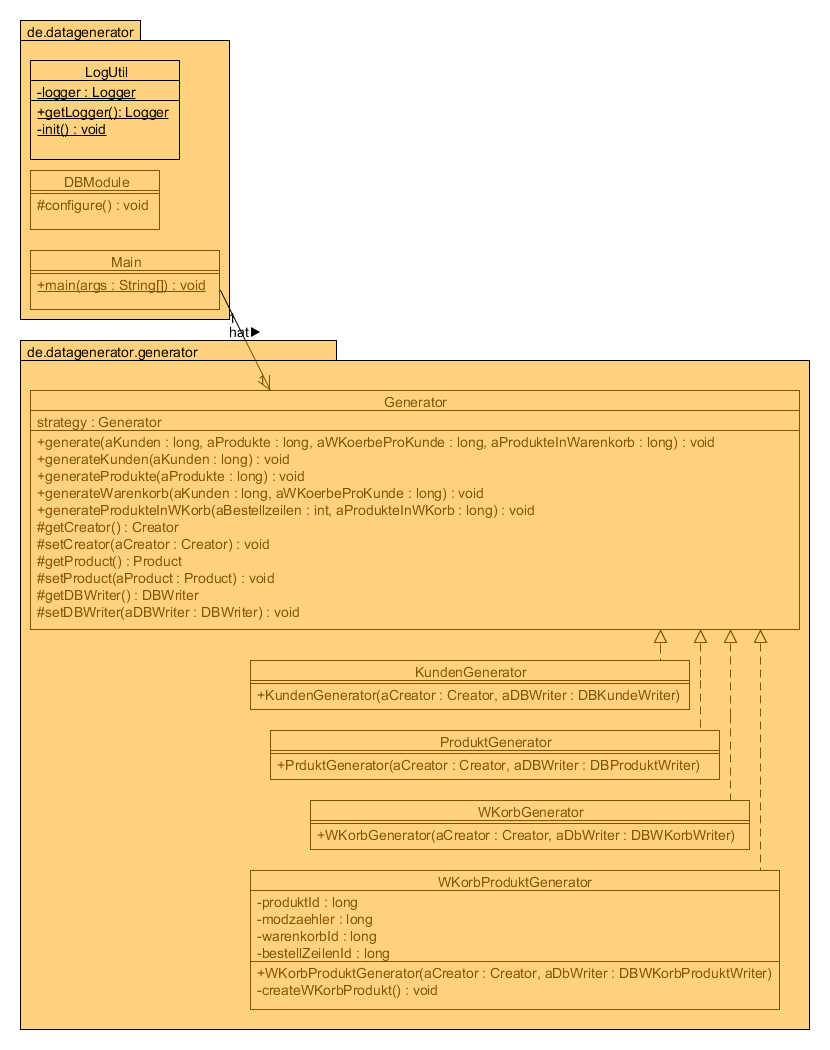
\includegraphics[width=1\textwidth]{Ingo/Bilder/EntwurfGeneratorkomponente.png}
\caption{Entwurf der Generatorkomponente}
\label{fig:EntwurfGeneratorkomponente}
\end{figure}

\subsection{Entwurfsklassendiagramm der DBWriterkomponente}
Abbildung \ref{fig:EntwurfDBWriterkomponente} auf Seite \pageref{fig:EntwurfDBWriterkomponente} zeigt das Entwurfsklassendiagramm der DBWriterkomponente.

\begin{figure}[htp]
\centering
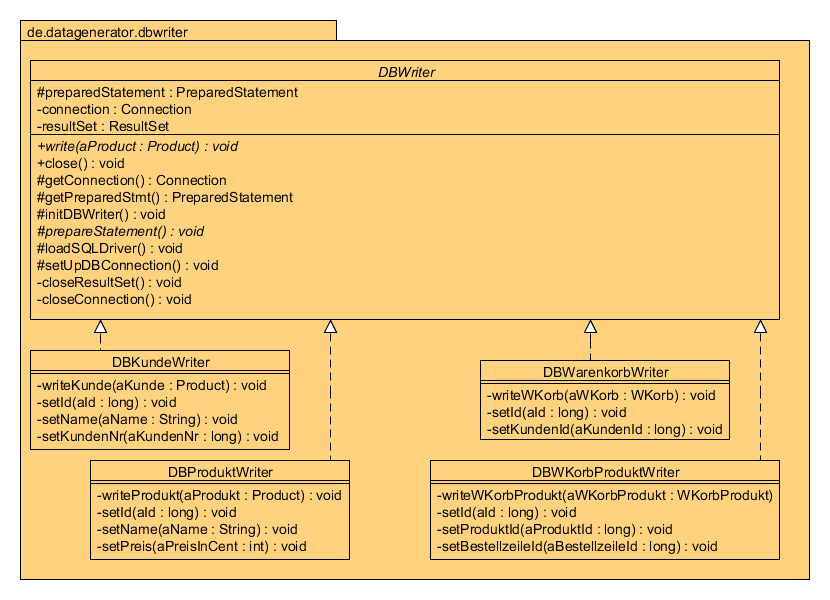
\includegraphics[width=1\textwidth]{Ingo/Bilder/EntwurfDBWriterkomponente.png}
\caption{Entwurf der DBWriterkomponente}
\label{fig:EntwurfDBWriterkomponente}
\end{figure}

\subsection{Entwurfsklassendiagramm der Creatorkomponente samt Datamodel}
Abbildung \ref{fig:EntwurfCreatorUndDatamodelKomponente} auf Seite \pageref{fig:EntwurfCreatorUndDatamodelKomponente} zeigt das Entwurfsklassendiagramm der Creatorkomponente und dem dazugeh�rigen Datamodel.

\begin{figure}[htp]
\centering
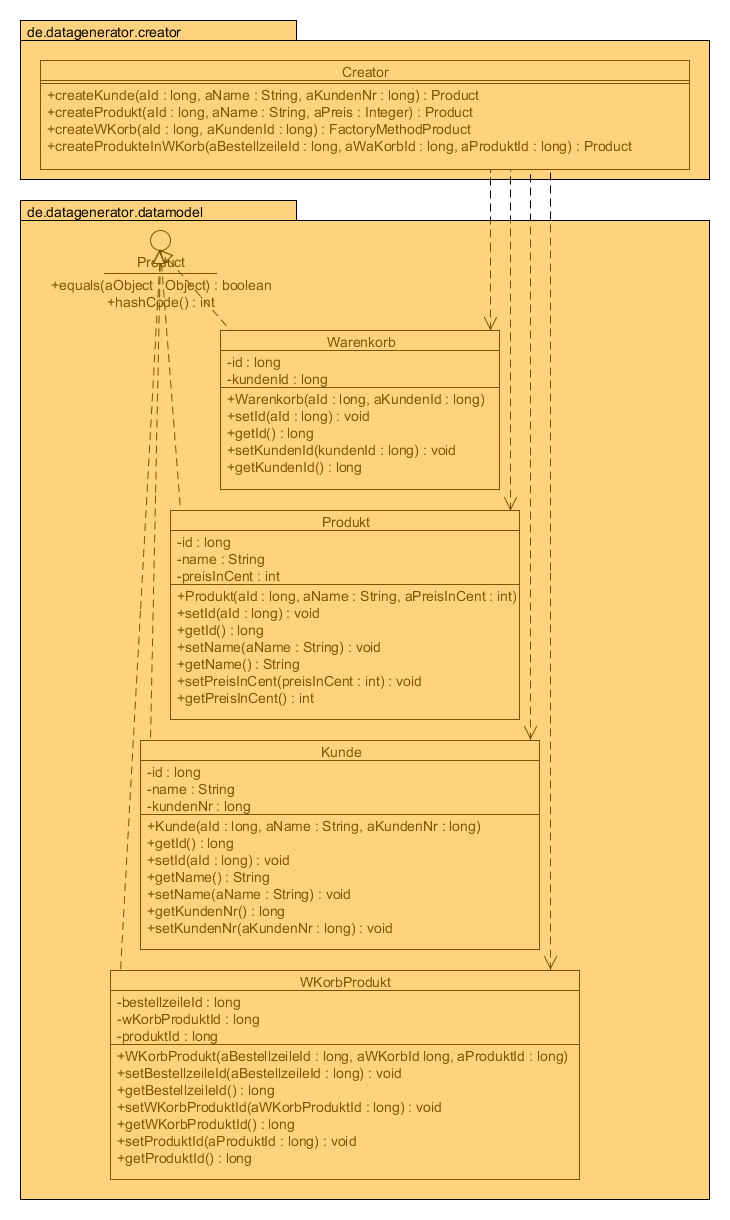
\includegraphics[width=0.9\textwidth]{Ingo/Bilder/EntwurfCreatorUndDatamodelKomponente.png}
\caption{Entwurf der Creatorkomponente}
\label{fig:EntwurfCreatorUndDatamodelKomponente}
\end{figure}

\subsection{Architektur}
Der Generator hat eine zweischichtige Architektur (two tier architecture). Die Komponente Generator greift auf die Dienste der Komponente DBWriter zu. Auch sonst wurde in der Anwendung auf geringe Kopplung geachtet.

\subsection{Prepared Statement}
Die generierten Testdaten werden �ber sogenannte Prepared Statements in die Tabellen geschrieben. Prepared Statements enthalten Platzhalter f�r die eigentlich zu schreibenden Daten. Prepared Statements bieten sich u.a. dann an, wenn sich bei dem Statement nur die Parameterwerte unterscheiden. Prepared Statements bringen einen Geschwindigkeitsvorteil, da sie bereits im DBMS vor�bersetzt werden und der DBWriter mit sehr viel generierten Parameterwerten aufgerufen wird.

\subsection{Entwurfsmuster}
Der Creator ist als einfache Fabrik implementiert. Durch ihn werden konkrete Instanziierungen aus dem Clientcode entfernt und somit die Clients von konkreten Klassen entkoppelt (Dependency Inversion Principle).

In z.B. DBWriter konnte initDBWriter() als Template Method implementiert werden. Sie definiert die Schritte f�r die Initialisierung eines DBWriters, wobei die Unterklassen entscheiden, wie sie die abstrakte Hook-Methode prepareStatement() implementieren. Durch die Template Method werden die Highlevel Komponenten loadSQLDriver() und setUpDBConnection() von Lowlevel Komponente prepareStatement() entkoppelt. Die Lowlevel-Komponenten prepareStatement() kann sich in initDBWriter() reinh�ngen, und die Highlevel Komponenten initDBWriter() bestimmt, wann und wie prepareStatement() aufgerufen wird. Die Lowlevel Komponente prepareStatement() ruft die Highlevel Komponente dabei nie direkt auf (Hollywood Prinzip).